\chapter{IMPLEMENTASI} \label{chap:implementasi}

\tab Pada bab ini dijelaskan mengenai implementasi dari perancangan struktur data dan algoritme untuk menyelesaikan permasalahan \problemDua{} sebagaimana yang telah dijelaskan pada Bab \ref{chap:analisis-perancangan-sistem}. Penjelasan implementasi terdiri dari penjelasan kelas dan fungsi yang dibuat, disertai dengan \textit{pseudocode} untuk masing-masing fungsi tersebut.

\section{Lingkungan Implementasi}
\tab Lingkungan implementasi dalam pembuatan Tugas Akhir ini meliputi perangkat keras dan perangkat lunak dengan spesifikasi sebagai berikut:

\begin{enumerate}
	\item Perangkat Keras:
	\begin{itemize}
		\item Prosesor 2.6 GHz Intel Core i5 (I5-4278U)
		\item Memori 8 GB 1600 MHz DDR3
	\end{itemize}
	\item Perangkat Lunak:
	\begin{itemize}
		\item Sistem operasi macOS Mojave Versi 10.14.5
		\item \textit{Text editor} Visual Studio Code Versi 1.33.1
		\item Bahasa Pemrograman Python 3.7.3
		\item Flask \textit{Microframework} 1.0.2
	\end{itemize}			
\end{enumerate}

\section{Implementasi \textit{Data Precomputing}}
\tab \textit{Data precomputing} merupakan pemrosesan tahap pertama dalam algoritme k-MPPTI yang bertujuan untuk mengolah \textit{dataset} produk $P$ dan preferensi pelanggan $C$ dengan jumlah data sebanyak $n$ dan ukuran dimensi sebesar $d$, menjadi sebuah $Pandora Box$ yang menyimpan skor kontribusi pasar semua produk pada setiap waktu. 

Algoritme ini diimplementasikan menggunakan paradigma pemrograman berorientasi objek, sehingga semua data dan fungsi dibungkus dalam kelas-kelas. Ada empat macam kelas yang diimplementasikan, yaitu kelas \textit{EventQueue}, \textit{PandoraBox}, \textit{ReverseSkyline}, dan \textit{DynamicSkyline}. 

\begin{figure}[H]
	\begin{algorithm}[H]
		\caption{Precomputing}
		\begin{algorithmic}[1]
			\Statex \textbf{Input \hskip1em :} product dataset $P$, customer dataset $C$ 
			\Statex \textbf{Output \hskip0.3em :} pandora box $PB$
			\State $EQ \leftarrow initEventQueue()$ 
			\State $D \leftarrow$ Data indexing $P, C$ 
			\ForAll {$d \in D$}
			\For {$i \leftarrow$ 0 to 2}
			\If {$i$ is 0} $enqueue(t_{in}, dt, id, i)$ to $EQ$
			\Else{} $enqueue(t_{out}, dt, id, i)$ to $EQ$
			\EndIf
			\EndFor
			\EndFor
			\State $sortQueue(EQ)$
			\State $PA \leftarrow \emptyset$ of active products
			\State $CA \leftarrow \emptyset$ of active customers
			\State $MaxTs \leftarrow$ get maximum timestamp 
			\State $MaxVal \leftarrow$ get maximum value 
			\State $PB \leftarrow$ new $initPandoraBox(Len(P), MaxTs)$ 
			\State $RSL \leftarrow$ new $initReverseSkyline(P, C, Dim)$
			\State $DSL \leftarrow$ new $initDynamicSkyline(P, C, Dim)$
			\algstore{main1}
		\end{algorithmic}
	\end{algorithm}
	\caption{Algoritme \textit{Precomputing} (Bagian 1) \label{algo:main-func-1}}
\end{figure}

\pagebreak
Secara garis besar, langkah yang dilakukan selama \textit{precomputing} adalah (1) \textit{indexing} data dan pembentukan \textit{EventQueue} (baris pertama hingga ke-tujuh pada Algoritme \ref{algo:main-func-1}), (2) inisialisasi dan instansiasi objek (baris ke-delapan hingga terakhir pada Algoritme \ref{algo:main-func-1}), dan (3) pemrosesan \textit{event} (Algoritme \ref{algo:main-func-3}).

\begin{figure}[H]
	\begin{algorithm}[H]
		\caption{Precomputing}
		\begin{algorithmic}[1]
			\algrestore{main1}
			\While {$EQ$ not $empty()$}
			\State $e \leftarrow dequeue(EQ)$
			\If {$e$ role is product}
			\If {$e$ action is insertion}  
			\State $PA \leftarrow$ append $p \in e$
			\State $RSL(p) \leftarrow computeRSL(p)$
			\ForAll {$c \in RSL(p)$ \textbf{parallel}}
			\State $DSL(c) \leftarrow computeDSL(c, ts, act, p)$
			\EndFor
			\ForAll {$c \in CA$ \textbf{parallel}}
			\State $updatePBox(DSL(c))$
			\EndFor
			\ElsIf {$e$ act is deletion}
			\ForAll {$c \in CA$ \textbf{parallel}}
			\State $DSL(c) \leftarrow updatePBox(DSL(c))$
			\EndFor
			\State $RSL(p) \leftarrow computeRSL(p)$
			\ForAll {$c \in RSL(p)$ \textbf{parallel}}
			\State $DSL(c) \leftarrow computeDSL(c, ts, act, p)$
			\EndFor
			\State $PA \leftarrow$ remove $p \in e$
			\EndIf
			\algstore{main2}
		\end{algorithmic}
	\end{algorithm}
	\caption{Algoritme \textit{Precomputing} (Bagian 2) \label{algo:main-func-2}}
\end{figure}
			
\begin{figure}[H]
	\begin{algorithm}[H]
		\caption{Precomputing}
		\begin{algorithmic}[1]
			\algrestore{main2}
			\ElsIf{$e$ role is customer}
			\If {$e$ act is insertion} 
			\State $CA \leftarrow$ append $c \in e$ 
			\State $DSL(c) \leftarrow computeDSL(c, ts)$
			\State $updatePBox(DSL(c))$
			\ElsIf {$e$ act is deletion}
			\State $DSL(c) \leftarrow computeDSL(c, ts)$
			\State $updatePBox(DSL(c))$
			\State $CA \leftarrow$ remove $c \in e$ 
			\EndIf
			\EndIf
			\EndWhile
		\end{algorithmic}
	\end{algorithm}
	\caption{Algoritme \textit{Precomputing} (Bagian 3) \label{algo:main-func-3}}
\end{figure}

\subsection{Kelas \textit{EventQueue}}
\tab Kelas \textit{EventQueue} mendefinisikan bentuk dan perilaku dari objek \textit{Event Queue} yang berfungsi untuk menyimpan \textit{event-event} yang terjadi di dalam himpunan data. \textit{EventQueue} tidak dibuat menggunakan struktur data \textit{queue} karena data yang digunakan adalah \textit{historical} dan diurutkan berdasarkan \textit{timestamp} dari data tersebut, bukan berdasarkan urutan masuknya data. Sehingga, \textit{EventQueue} diimplementasikan menggunakan \textit{array} yang bekerja seperti \textit{queue}, yakni FIFO (\textit{First In First Out}). 

Ada enam fungsi yang diimplementasikan dalam kelas ini sebagaimana yang ditunjukkan oleh Algoritme \ref{algo:event-queue-class}, namun hanya ada tiga fungsi utama, yaitu $enqueue$ untuk memasukkan data ke dalam \textit{array} pada indeks pertama, $dequeue$ untuk mengeluarkan data dari \textit{array} pada indeks terakhir; dan $sortQueue$ untuk mengurutkan data di dalam array.


\begin{figure}[H]
	\begin{algorithm}[H]
		\caption{EventQueue Class}
		\begin{algorithmic}[1]
			\Statex \textbf{Input \hskip1em :} timestamp $t$, role $o$ (product/customer), data ID $oid$, action $a$ (insertion/deletion)
			\Statex \textbf{Output \hskip0.3em :} event queue $E$
			\Procedure{$initEventQueue$}{}
			\State $E \leftarrow \emptyset$
			\EndProcedure
			\Procedure{$enqueue$}{$t$, $o$, $oid$, $a$}
			\State $e \leftarrow$ [$t, o, oid, a$]
			\State $E \leftarrow$ append $e$ 
			\EndProcedure
			\Procedure{$dequeue$}{}
			\State $e \leftarrow$ pop an element from $E$
			\State \Return $e$
			\EndProcedure
			\Procedure{$sortQueue$}{}
			\State $E \leftarrow$ sort elements in descending order based on sorting priority (timestamp, insertion act, deletion act, product, customer, data ID))
			\EndProcedure
			\Procedure{$getTotalQueue$}{}
			\State \Return number of elements in $E$
			\EndProcedure
			\Procedure{$getMaxTimestamp$}{}
			\State \Return timestamp in the first index of $E$ (descending order)
			\EndProcedure
			\Procedure{$getMinTimestamp$}{}
			\State \Return timestamp in last first index of $E$ (descending order)
			\EndProcedure
			\Procedure{$empty$}{}
			\If {$E$ is empty} \Return True
			\Else {} \Return False
			\EndIf
			\EndProcedure
		\end{algorithmic}
	\end{algorithm}
	\caption{Kelas \textit{EventQueue} \label{algo:event-queue-class}}
\end{figure}

\pagebreak
\subsection{Kelas \textit{PandoraBox}}
\tab Kelas \textit{PandoraBox} mendefinisikan bentuk dan perilaku dari objek \textit{Pandora Box} yang berfungsi untuk menyimpan skor kontribusi pasar masing-masing produk $p \in P$ pada setiap waktu dalam interval hidupnya $t \in [t_i:t_e]$. \textit{PandoraBox} diimplementasikan menggunakan struktur data \textit{array} dua dimensi, yaitu ID produk dan \textit{timestamp}.

\begin{figure}[H]
	\begin{algorithm}[H]
		\caption{PandoraBox Class}
		\begin{algorithmic}[1]
			\Statex \textbf{Input \hskip1em :} $DSL(c)$, timestamp now $ts$, probability score $pr$, last timestamp $lts$, last probability score $lpr$
			\Statex \textbf{Output \hskip0.3em :} filled pandora box $PBox$
			\Procedure{$initPandoraBox$}{}
			\State $PBox \leftarrow \emptyset$
			\EndProcedure
			\Procedure{$updatePBox$}{$DSL(c)$}
			\ForAll {$p \in DSL(c)$}
			\If{$ts > lts$}
			\State $updateScore(p, ts, pr, lts, lpr)$
			\Else
			\State $PBox(p, ts) \leftarrow PBox(p, ts) + pr$  
			\EndIf
			\EndFor
			\EndProcedure
			\Procedure{$updateScore$}{$p$, $ts$, $lts$, $pr$, $lpr$}
			\For {$i \leftarrow lts+1$ to $ts$}
			\State $PBox(p, i) \leftarrow PBox(p, i) + lpr$  
			\EndFor
			\State $PBox(p, i) \leftarrow PBox(p, i) + pr$
			\EndProcedure
			\algstore{pbox}
		\end{algorithmic}
	\end{algorithm}
	\caption{Kelas \textit{PandoraBox} (Bagian 1) \label{algo:pbox-class}}
\end{figure}

\pagebreak
Ada dua fungsi utama yang digunakan dalam proses \textit{data precomputing}, yaitu $updatePBox$ untuk memperbarui skor kontribusi pasar pelanggan $c$ dan $updateScore$ untuk memperbarui "kotak" sebelumnya menggunakan nilai probabilitas terakhir. Kelas \textit{Pandora Box} ditunjukkan oleh Algoritme \ref{algo:pbox-class}.

\subsection{Kelas \textit{ReverseSkyline}}
\tab Kelas \textit{ReverseSkyline} mendefinisikan bentuk dan perilaku dari objek \textit{Reverse Skyline} yang berfungsi untuk menangani komputasi \textit{reverse skyline}, meliputi (1) pembentukan \textit{orthant} pada fungsi $defineOrthant$ dan $getOrthantId$, (2) menghitung \textit{midpoint} antara produk kueri dan produk lainnya pada fungsi $calcMidpoint$, (3) menentukan \textit{midpoint skyline} masing-masing \textit{orthant} pada fungsi $findMidSkyline$, dan (4) menentukan \textit{reverse skyline} pada fungsi $findReverseSkyline$. Kelas \textit{ReverseSkyline} ditunjukkan pada Algoritme \ref{algo:rsl-class-1}, \ref{algo:rsl-class-2}, \ref{algo:rsl-class-3}.

\begin{figure}[H]
	\begin{algorithm}[H]
		\caption{ReverseSkyline Class}
		\begin{algorithmic}[1]
			\Statex \textbf{Input \hskip1em :} product as query point $p_q$, active products $PA$, active customers $CA$
			\Statex \textbf{Output \hskip0.3em :} $RSL(p)$
			\Procedure{$initReverseSkyline$}{$P$, $C$, $d$}
			\State $PA \leftarrow$ get product active from $P$
			\State $CA \leftarrow$ get customer active from $C$
			\State $O \leftarrow defineOrthant(Dim)$
			\EndProcedure
			\Procedure{$computeRSL$}{$p_q$}
			\State $findMidSkyline(p_q, PA)$
			\State $RSL(p) \leftarrow findReverseSkyline(CA)$
			\EndProcedure
			\algstore{rsl}
		\end{algorithmic}
	\end{algorithm}
	\caption{Kelas \textit{ReverseSkyline} (Bagian 1) \label{algo:rsl-class-1}}
\end{figure}

\begin{figure}[H]
	\begin{algorithm}[H]
		\caption{ReverseSkyline Class}
		\begin{algorithmic}[1]
			\algrestore{rsl}
			\Procedure{$findMidSkyline$}{$p_q, PA$}
			\ForAll {$p \in PA$}
			\If {$p \not= p_q$}
			\State $m \leftarrow calcMidpoint(p_q, p)$ 
			\State $id \leftarrow getOrthantId(p)$
			\If {$O_{id}$ is empty} $O_{id} \leftarrow m$
			\Else{} 
			\For {\textbf{each} $ms \in MSL(o)$}
			\If{$m \prec ms$} 
			\State $MSL(o) \leftarrow$ delete $ms$
			\ElsIf{$ms \prec m$}
			\State exit the loop 
			\EndIf
			\If{$m \nprec ms$}
			\State $MSL(o) \leftarrow$ insert $m$
			\EndIf
			\EndFor
			\EndIf
			\EndIf
			\EndFor
			\EndProcedure
			\Procedure{$findReverseSkyline$}{$CA$} 
			\State $RSL(p) \leftarrow \emptyset$
			\For {$c \in CA$}
			\State $id \leftarrow$ $getOrthantId(c)$
			\If {$O_{id}$ is empty} 
			\State $RSL(p) \leftarrow$ insert $c$
			\Else{}  
			\State $dom \leftarrow 0$
			\ForAll {$m \in O_{id}$}
			\If {$m \prec c$}
			\State $dom \leftarrow dom + 1$						
			\EndIf
			\EndFor
			\If {$dom$ is $0$}
			\State $RSL(p) \leftarrow$ insert $c$
			\EndIf
			\EndIf
			\EndFor
			\State \Return $RSL(p)$
			\EndProcedure
			\algstore{rsl1}
		\end{algorithmic}
	\end{algorithm}
	\caption{Kelas \textit{ReverseSkyline} (Bagian 2) \label{algo:rsl-class-2}}
\end{figure}

\begin{figure}[H]
	\begin{algorithm}[H]
		\caption{ReverseSkyline Class}
		\begin{algorithmic}[1]
			\algrestore{rsl1}
			\Procedure{$calcMidpoint$}{$p_q$, $p$} 
			\State $m \leftarrow \emptyset$
			\For {\textbf{each} $i \in d$} $m \leftarrow$ $\frac{(p_q^i + p^i)}{2}$
			\EndFor
			\State \Return $m$
			\EndProcedure
			\Procedure{$getOrthantId$}{$D$}
			\State $o \leftarrow \varnothing$
			\For {\textbf{each} $i \in d$}
			\If {$D^i \leq p_q^i$} $o \leftarrow$ append $0$
			\Else {} $o \leftarrow$ append $1$
			\EndIf
			\EndFor
			\State \Return $o$
			\EndProcedure
		\end{algorithmic}
	\end{algorithm}
	\caption{Kelas \textit{ReverseSkyline} (Bagian 3) \label{algo:rsl-class-3}}
\end{figure}

\subsection{Kelas \textit{Dynamic Skyline}}
\tab Kelas \textit{DynamicSkyline} mendefinisikan bentuk dan perilaku dari objek \textit{Dynamic Skyline} yang berfungsi untuk menangani komputasi \textit{dynamic skyline} yang memiliki 3 jenis pemrosesan \textit{event}, yaitu (1) \textit{Initial} $DSL$, digunakan ketika ada data pelanggan yang masuk (\textit{customer insertion}), (2) $DSL-PI$, digunakan ketika ada data produk yang masuk (\textit{product insertion}), dan (3) $DSL-PD$, digunakan ketika ada data produk yang keluar (\textit{product deletion}). Kelas \textit{DynamicSkyline} ditunjukkan pada Algoritme \ref{algo:dsl-class-1} dan \ref{algo:dsl-class-2}.

\begin{figure}[H]
	\begin{algorithm}[H]
		\caption{DynamicSkyline Class}
		\begin{algorithmic}[1]
			\Statex \textbf{Input \hskip1em :} customer $c$, product data $P$ 
			\Statex \textbf{Output \hskip0.3em :} $DSL(p)$
			\Procedure{$initDynamicSkyline$}{$P$, $C$, $d$}
			\State $PA \leftarrow$ get product active from $P$
			\EndProcedure
			\Procedure{$computeDSL$}{$c$, $ts$, $act$, $p$}
			\If{$act$ is customer insertion}
			\State $initDSL(c, ts)$
			\ElsIf{$act$ is product insertion}
			\State $productIn(c, ts, p)$
			\ElsIf{$act$ is product deletion}
			\State $productOut(c, ts, p)$
			\EndIf
			\EndProcedure
			\Procedure{$initDSl$}{$c$}
			\State $CAND \leftarrow PA$
			\State sort $CAND$
			\For {$i \leftarrow$ 0 to length of $CAND$}
			\For {$j \leftarrow i + 1$ to length of $CAND$}
			\If {$p_i \prec p_j$} 
			\State add $p_j$ to the child list of $p_i$
			\State $CAND \leftarrow$ remove $p_j$
			\ElsIf {$p_j \prec p_i$} 
			\State add $p_i$ to the child list of $p_j$
			\State $CAND \leftarrow$ remove $p_i$
			\State break the loop
			\EndIf
			\EndFor
			\State \Return $CAND$ as $DSL(c)$
			\EndFor
			\EndProcedure
			\algstore{dsl}
		\end{algorithmic}
	\end{algorithm}
	\caption{Kelas \textit{DynamicSkyline} (Bagian 1) \label{algo:dsl-class-1}}
\end{figure}

\begin{figure}[H]
	\begin{algorithm}[H]
		\caption{DynamicSkyline Class}
		\begin{algorithmic}[1]
			\algrestore{dsl}
			\Procedure{$productIn$}{$p$}
			\State $CAND \leftarrow p, DSL(c)$
			\State sort $CAND$
			\State $index \leftarrow$ get index of p in $CAND$
			\For {$i \leftarrow$ 0 to length of $CAND$}
				\If{$i < index$}
					\If {$p_i \prec p_{index}$} 
					\State add $p_{index}$ to the child list of $p_i$
					\State $CAND \leftarrow$ remove $p_{index}$
					\State break the loop
					\EndIf
				\ElsIf{$i > index$}
					\If {$p_{index} \prec p_i$} 
					\State add $p_i$ to the child list of $p_{index}$
					\State $CAND \leftarrow$ remove $p_i$
					\EndIf
				\EndIf
			\EndFor
			\State \Return $CAND$ as $DSL(c)$
			\EndProcedure
			\Procedure{$productOut$}{$p$}
			\State $AC \leftarrow$ find active childs of $p$
			\State $DSL(c) \leftarrow productIn(AC)$  
			\State \Return $DSL(c)$
			\EndProcedure
		\end{algorithmic}
	\end{algorithm}
	\caption{Kelas \textit{DynamicSkyline} (Bagian 2) \label{algo:dsl-class-2}}
\end{figure}

\begin{figure}[H]
	\begin{algorithm}[H]
		\caption{Check Domination}
		\begin{algorithmic}[1]
			\Statex \textbf{Input \hskip1em :} value of subject ($val_s$), value of target ($val_t$), value of query point ($val_q$), dimension of data ($d$)
			\Statex \textbf{Output \hskip0.3em :} is subject dominating target based on query point? ($s \prec_q t$)
			\Procedure{$isDominating$}{$val_s, val_t, val_q$} 
			\State $dg \leftarrow 0$ \Comment{counter of dominating}
			\State $dd \leftarrow 0$ \Comment{counter of dominated}
			\For {\textbf{each} $i \in d$}
			\State $diff_s^i \leftarrow |val_s^i - val_q^i|$
			\State $diff_t^i \leftarrow |val_t^i - val_q^i|$
			\If {$diff_a^i = diff_b^i$}
			\State \textbf{continue the loop}
			\ElsIf{$diff_s^i < diff_t^i$}
			\State $dg \leftarrow dg+1$
			\ElsIf{$diff_s^i > diff_t^i$}
			\State $dd \leftarrow dd+1$
			\EndIf
			\EndFor
			\If{$dd = 0$ and $dg \geq 1$} 
			\State \Return True
			\Else{} 
			\State \Return False
			\EndIf
			\EndProcedure
		\end{algorithmic}
	\end{algorithm}
	\caption{Fungsi \textit{Check Domination} \label{algo:check-dom}}
\end{figure}

\section{Implementasi Algoritme \textit{Query Processing}}
\tab \textit{Query processing} merupakan pemrosesan tahap kedua dalam algoritme k-MPPTI yang bertujuan untuk memproses kueri yang dimasukkan oleh pengguna dengan memanfaatkan \textit{Pandora Box} dari hasil \textit{precomputing}. Proses diawali dengan mengakumulasi skor kontribusi pasar semua produk dalam interval waktu kueri, kemudian hasil akumulasi diurutkan dari yang terbesar. Langkah terakhir adalah mengembalikan hasil kueri berupa produk sejumlah $k$ beserta skor kontribusi pasarnya.

\begin{figure}[H]
	\begin{algorithm}[H]
		\caption{Solution}
		\begin{algorithmic}[1]
			\Statex \textbf{Input \hskip1em :} Pandora Box $PBox$, number of products $k$, time interval (time init $t_i$, time end $t_e$)
			\Statex \textbf{Output \hskip0.3em :} $k$ products
			\Procedure{$solution$}{$PBox$, $k$, $t_i$, $t_e$}
			\State $Res \leftarrow \emptyset$
			\ForAll {$p \in P$}
			\State $MC(p) \leftarrow getScore(p, t_i, t_e)$
			\EndFor
			\State sort $MC$ in ascending order
			\For{$i \leftarrow$ 0 to $k$}
			\State $Res \leftarrow$ append $MC(i)$
			\EndFor
			\Return $Res$
			\EndProcedure
		\end{algorithmic}
	\end{algorithm}
	\caption{Algoritme \textit{Solutio} \label{algo:solution}}
\end{figure}

\begin{figure}[H]
	\begin{algorithm}[H]
		\caption{PandoraBox Class}
		\begin{algorithmic}[1]
			\algrestore{pbox}
			\Statex \textbf{Input \hskip1em :} product $p$, time interval (time init $t_i$, time end $t_e$)
			\Statex \textbf{Output \hskip0.3em :} total market contribution score $MC$
			\Procedure{$getScore$}{$p[id]$, $t_i$, $t_e$}
			\State $MC \leftarrow 0$ 
			\For {$i \leftarrow t_i$ to $t_e + 1$}
			\State $MC \leftarrow MC + PBox(p, i)$
			\EndFor
			\Return $MC$
			\EndProcedure
		\end{algorithmic}
	\end{algorithm}
	\caption{Kelas \textit{PandoraBox} (Bagian 2) \label{algo:pbox-class-2}}
\end{figure}

\section{Implementasi Antarmuka Pengguna}
\tab Antarmuka pengguna diimplementasikan menggunakan bahasa pemrograman Python, HTML, CSS, dan JavaScript, serta Flask sebagai kerangka kerja \textit{back-end}, Bootstrap sebagai kerangka kerja \textit{front-end}, dan pustaka Vis.js untuk menampilkan visualisasi data. 

\begin{figure}[H]
	\centering
	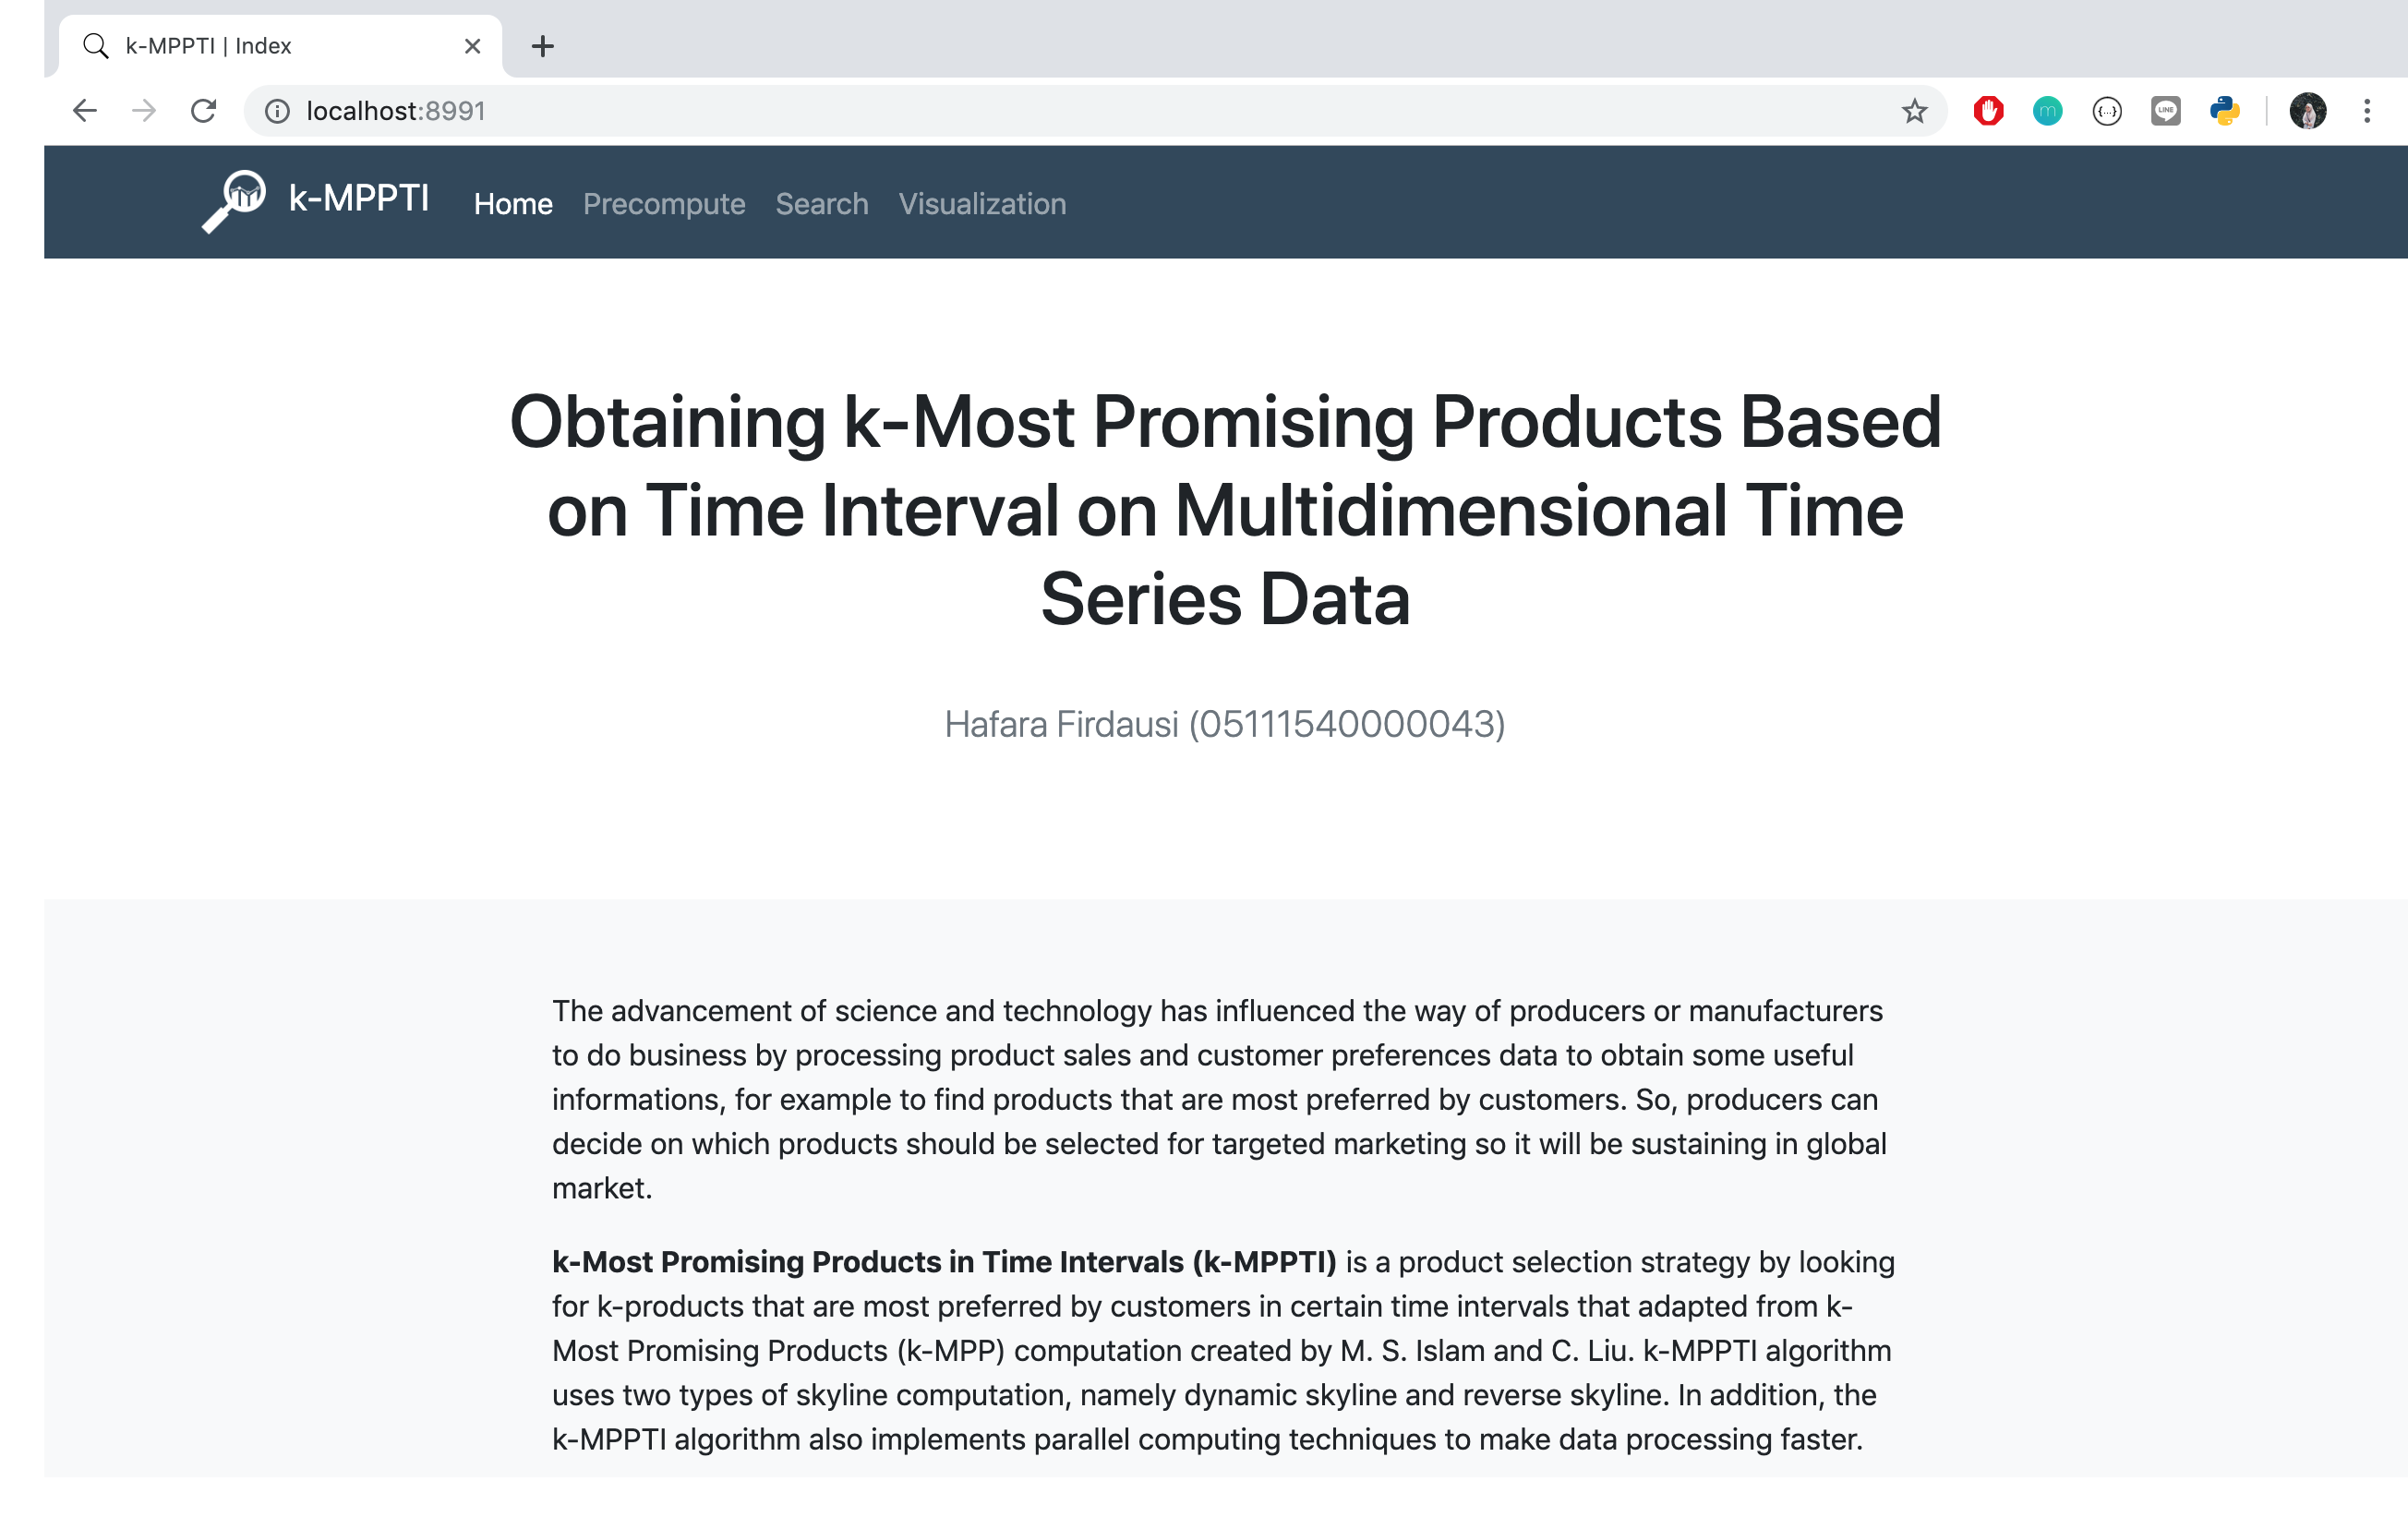
\includegraphics[width=8cm]{assets/img/bab4/home.png}
	\caption{Implementasi Halaman \textit{Home}}
	\label{fig:home}
\end{figure}

\begin{figure}[H]
	\centering
	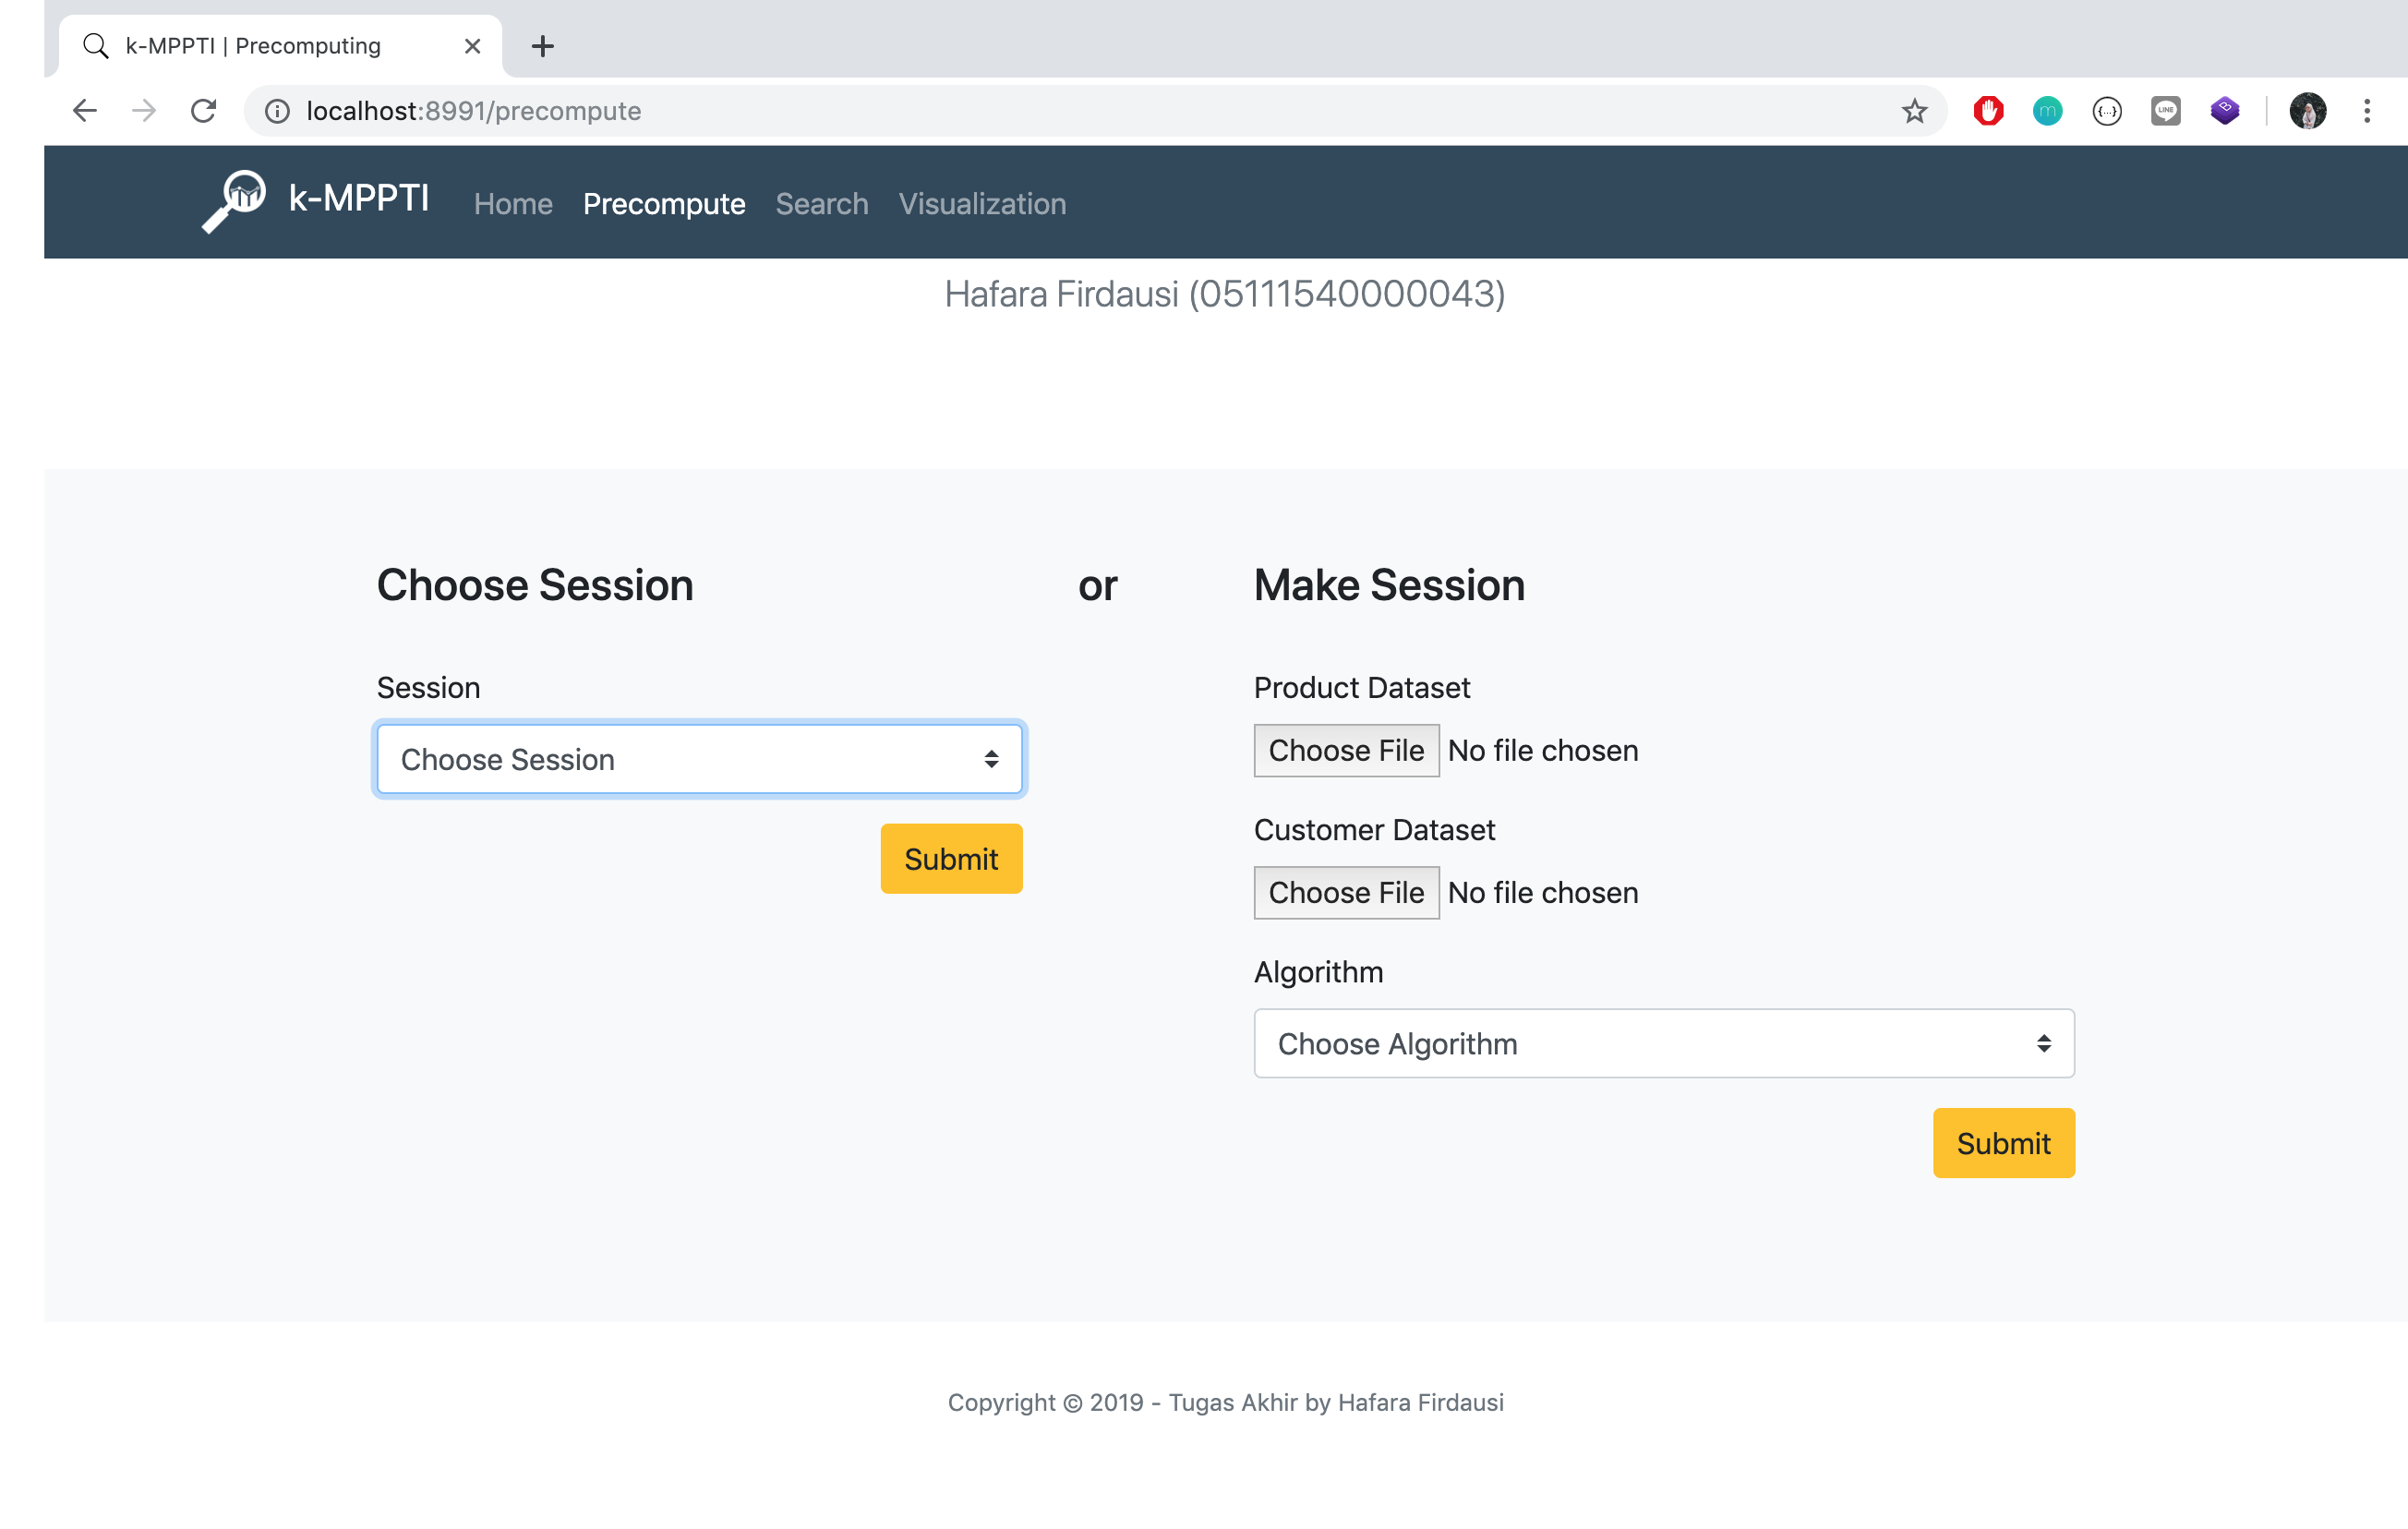
\includegraphics[width=8cm]{assets/img/bab4/precompute.png}
	\caption{Implementasi Halaman \textit{Precompute}}
	\label{fig:precompute}
\end{figure}

Antarmuka pengguna memiliki empat menu utama yaitu, \textit{"Home"} sebagai halaman utama yang berisi pengenalan algoritme k-MPPTI, \textit{"Precompute"} untuk melakukan \textit{data precomputing}, \textit{"Search"} untuk melakukan pencarian $k$-produk yang paling diminati pelanggan dalam interval waktu tertentu, dan \textit{"Visualization"} untuk melihat visualisasi data.

Pada menu \textit{"Precompute"} (Gambar \ref{fig:precompute}), pengguna diberikan opsi untuk memasukkan data baru atau menggunakan \textit{session} yang sudah ada. Jika pengguna memasukkan data baru, artinya pengguna membuat \textit{session} baru dan data akan di-\textit{precompute} terlebih dahulu. Jika pengguna memilih session yang sudah ada, data tidak perlu di-\textit{precompute} ulang.

\begin{figure}[H]
	\centering
	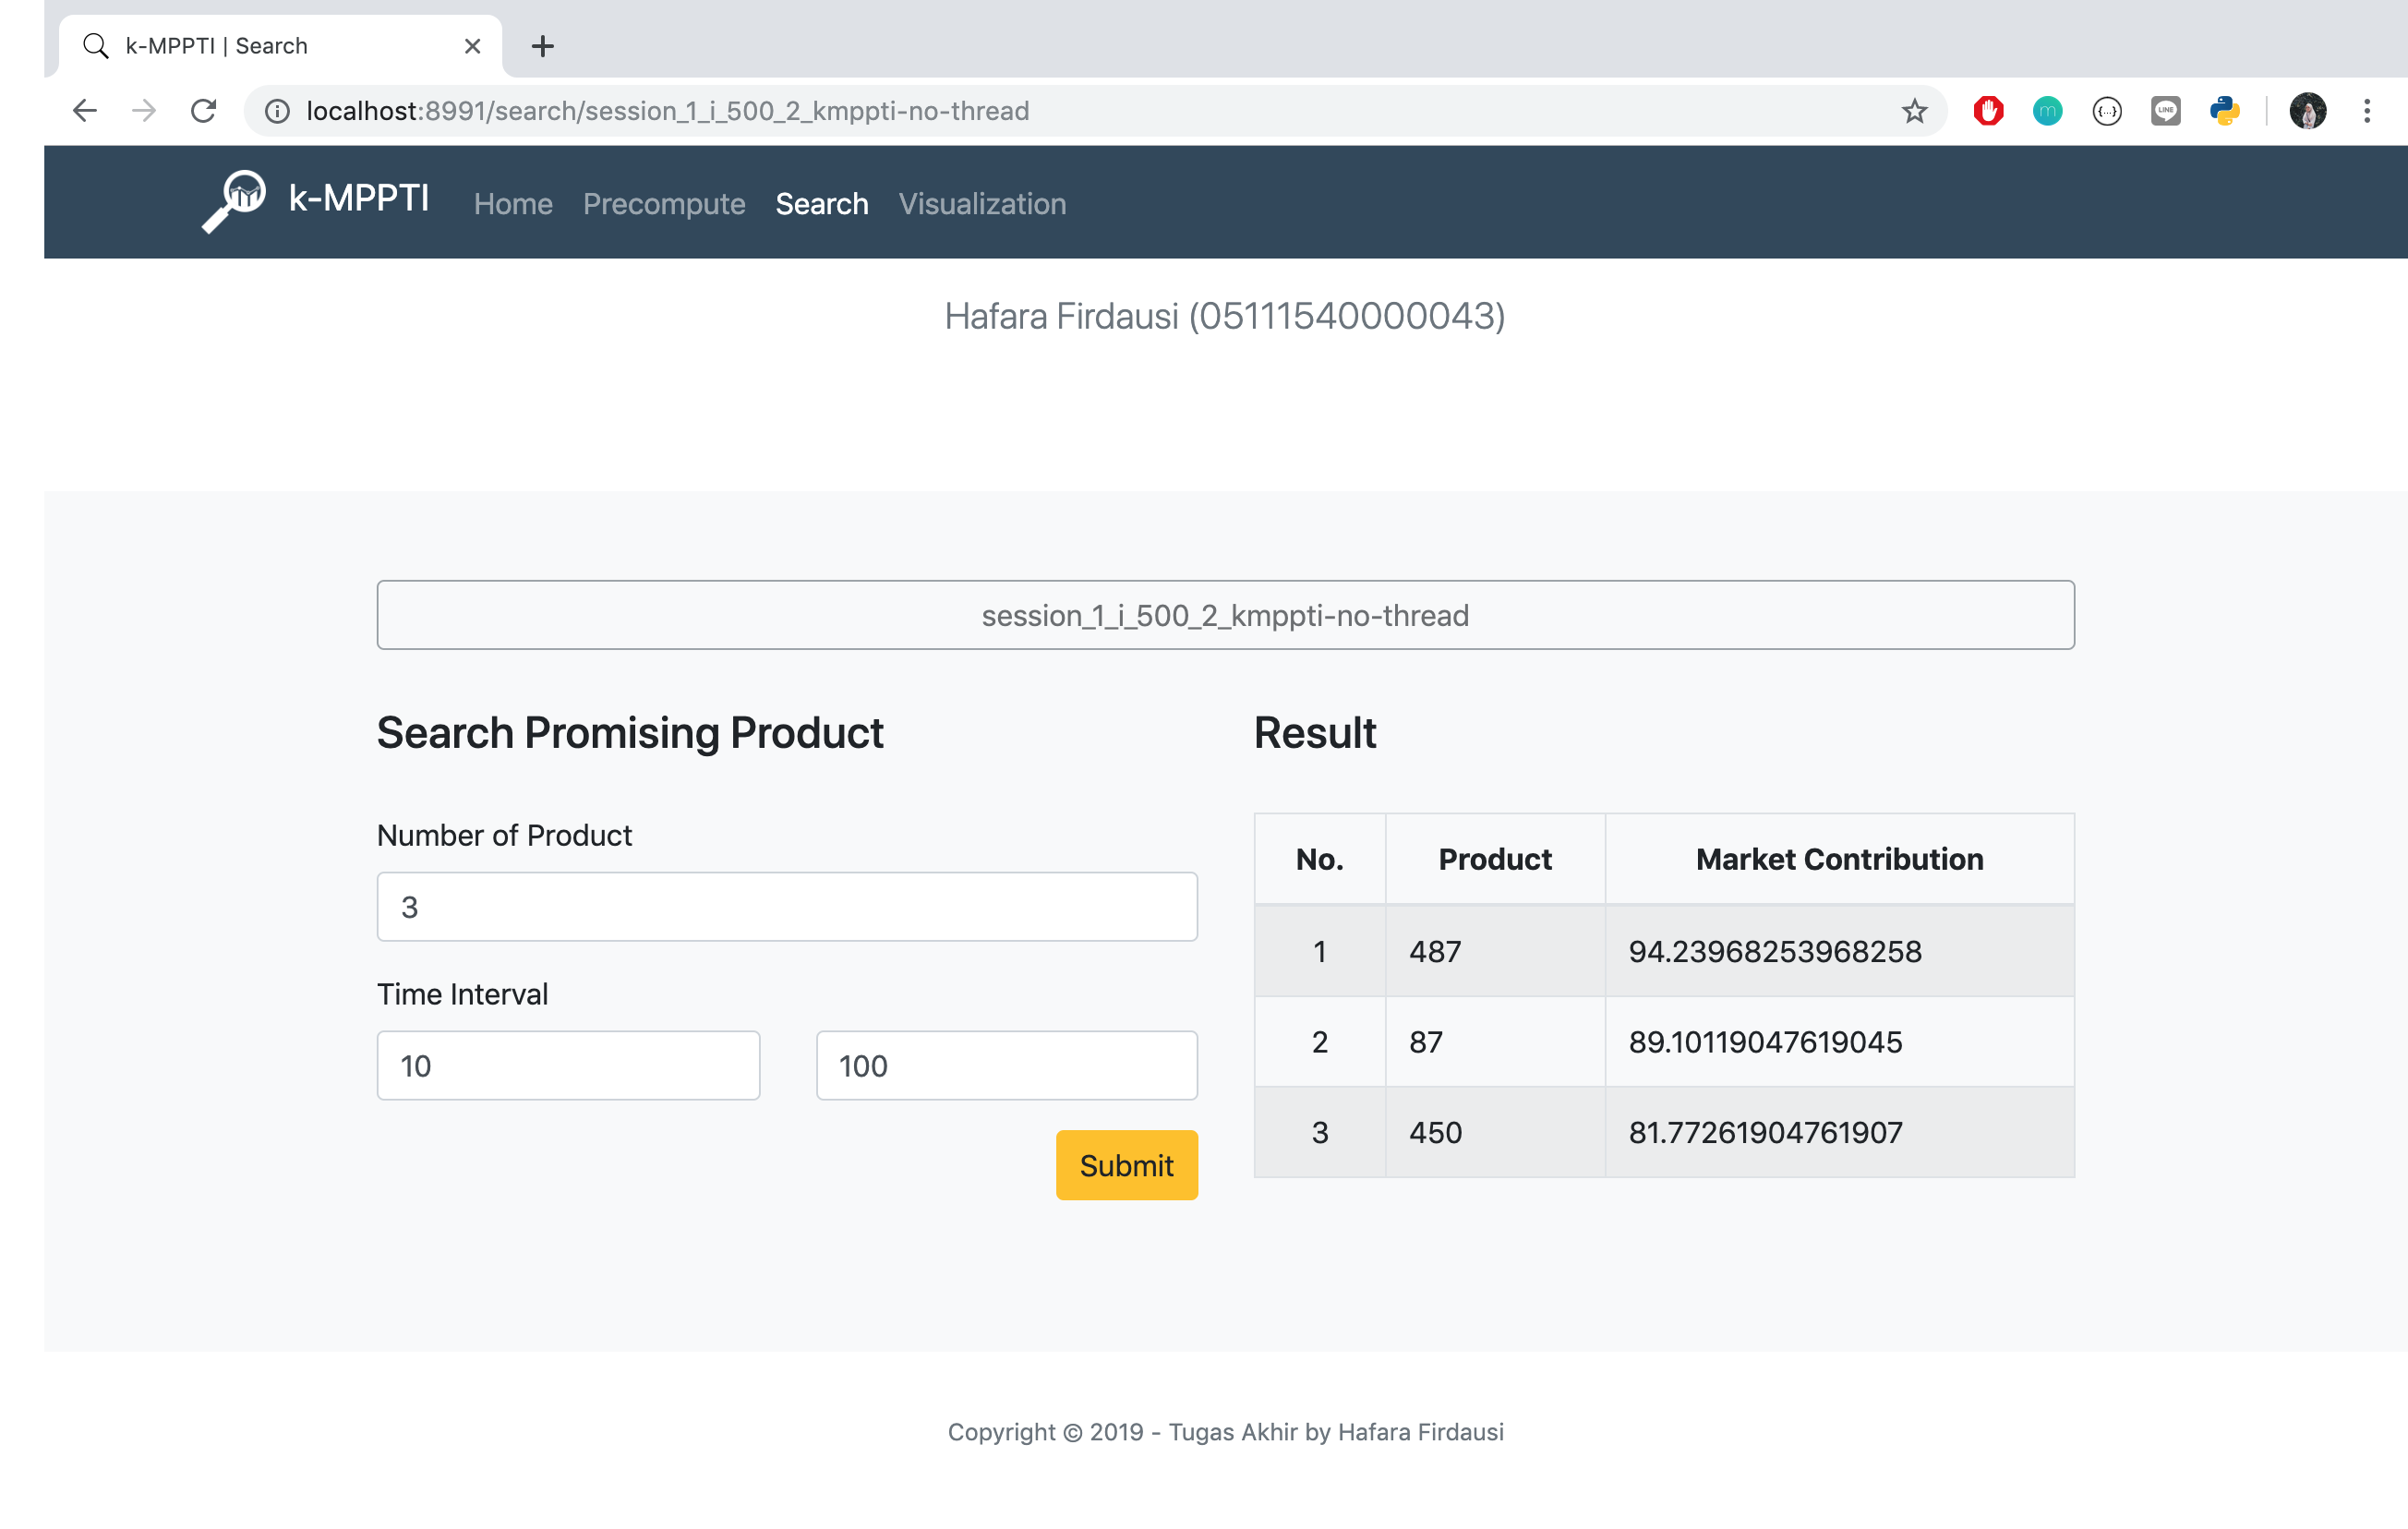
\includegraphics[width=8cm]{assets/img/bab4/search.png}
	\caption{Implementasi Halaman \textit{Search}}
	\label{fig:search}
\end{figure}

Setelah melalui proses \textit{precomputing}, pengguna dapat memasukkan kueri pencarian $k$-produk yang paling menjanjikan dalam interval waktu tertentu. Halaman web akan mengembalikan data berupa hasil kueri pencarian, yakni berupa ID produk dan skor kontribusi pasarnya sebagaimana yang ditunjukkan pada Gambar \ref{fig:search}.

Pengguna juga dapat melihat visualisasi data pada menu \textit{"Visualization"} berupa pratinjau data dalam bentuk tabel dan lini masa. Selain itu, pengguna juga dapat melihat informasi detail dari data. Berikut adalah beberapa cuplikan tampilan visualisasi data pada Gambar \ref{fig:visual-data-info}, \ref{fig:visual-table}, dan \ref{fig:visual-timeline}.

\begin{figure}[H]
	\centering
	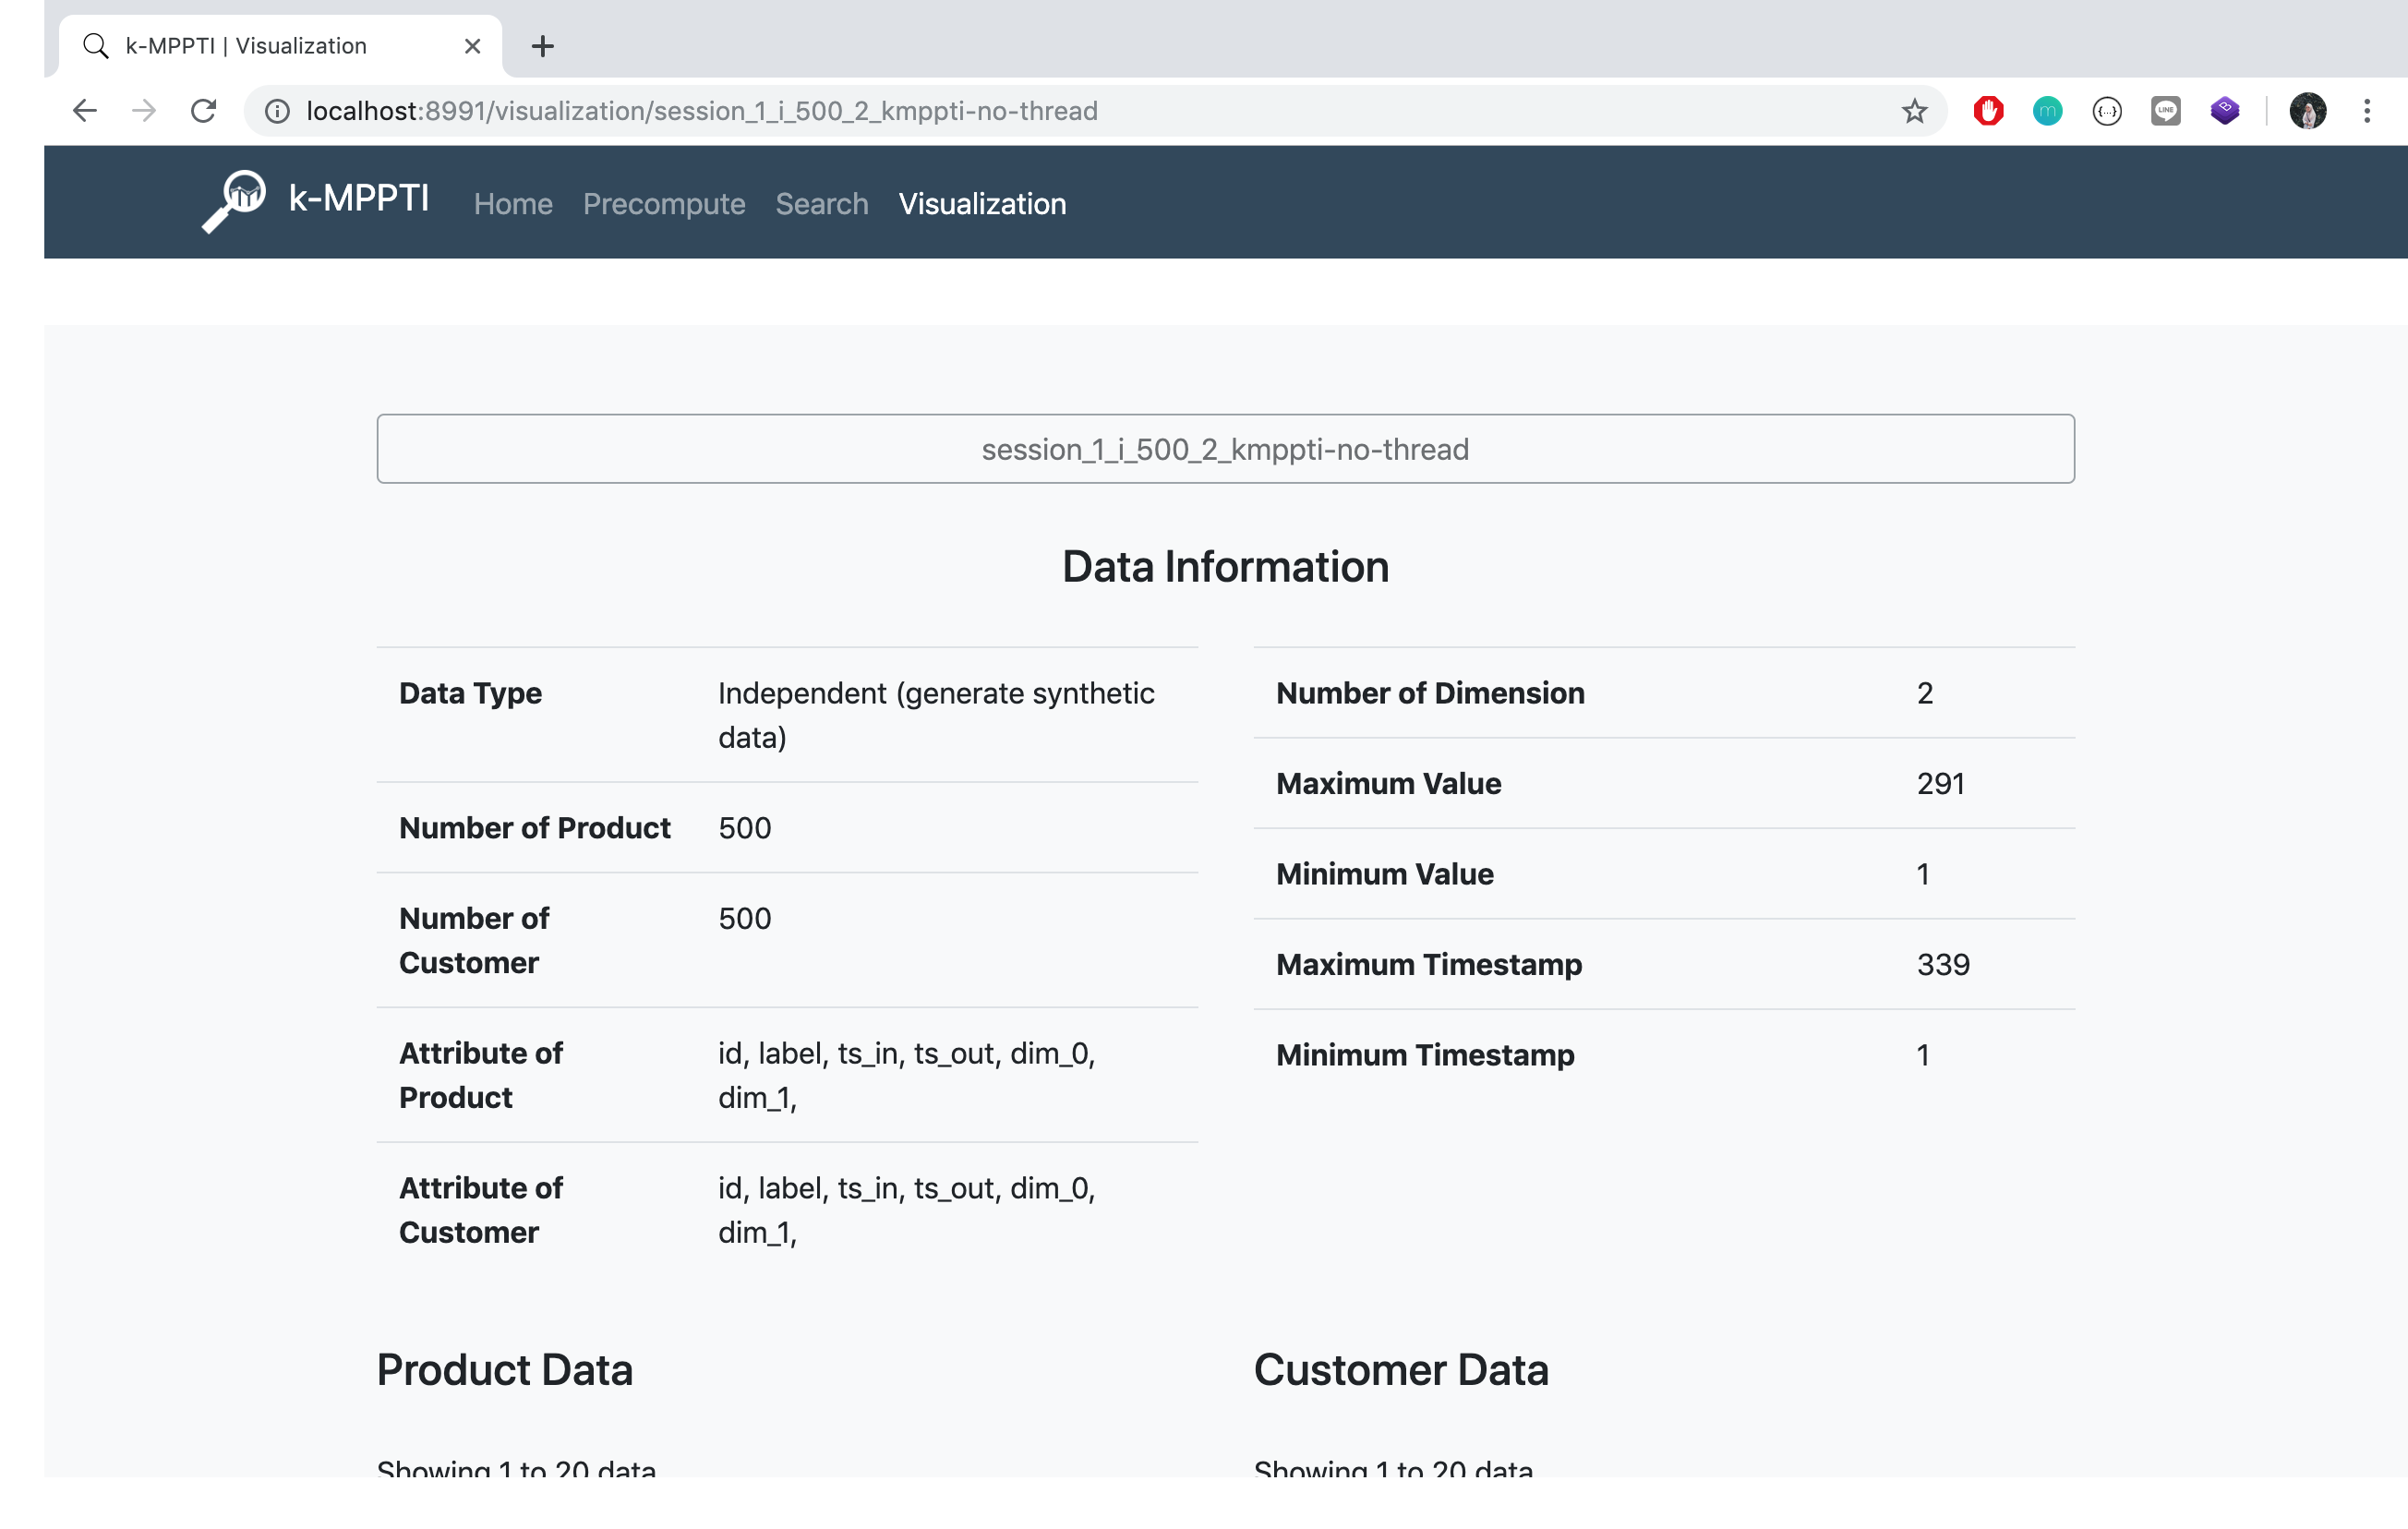
\includegraphics[width=8cm]{assets/img/bab4/data-info.png}
	\caption{Implementasi Halaman \textit{Visualization} (Informasi Data)}
	\label{fig:visual-data-info}
\end{figure}

\begin{figure}[H]
	\centering
	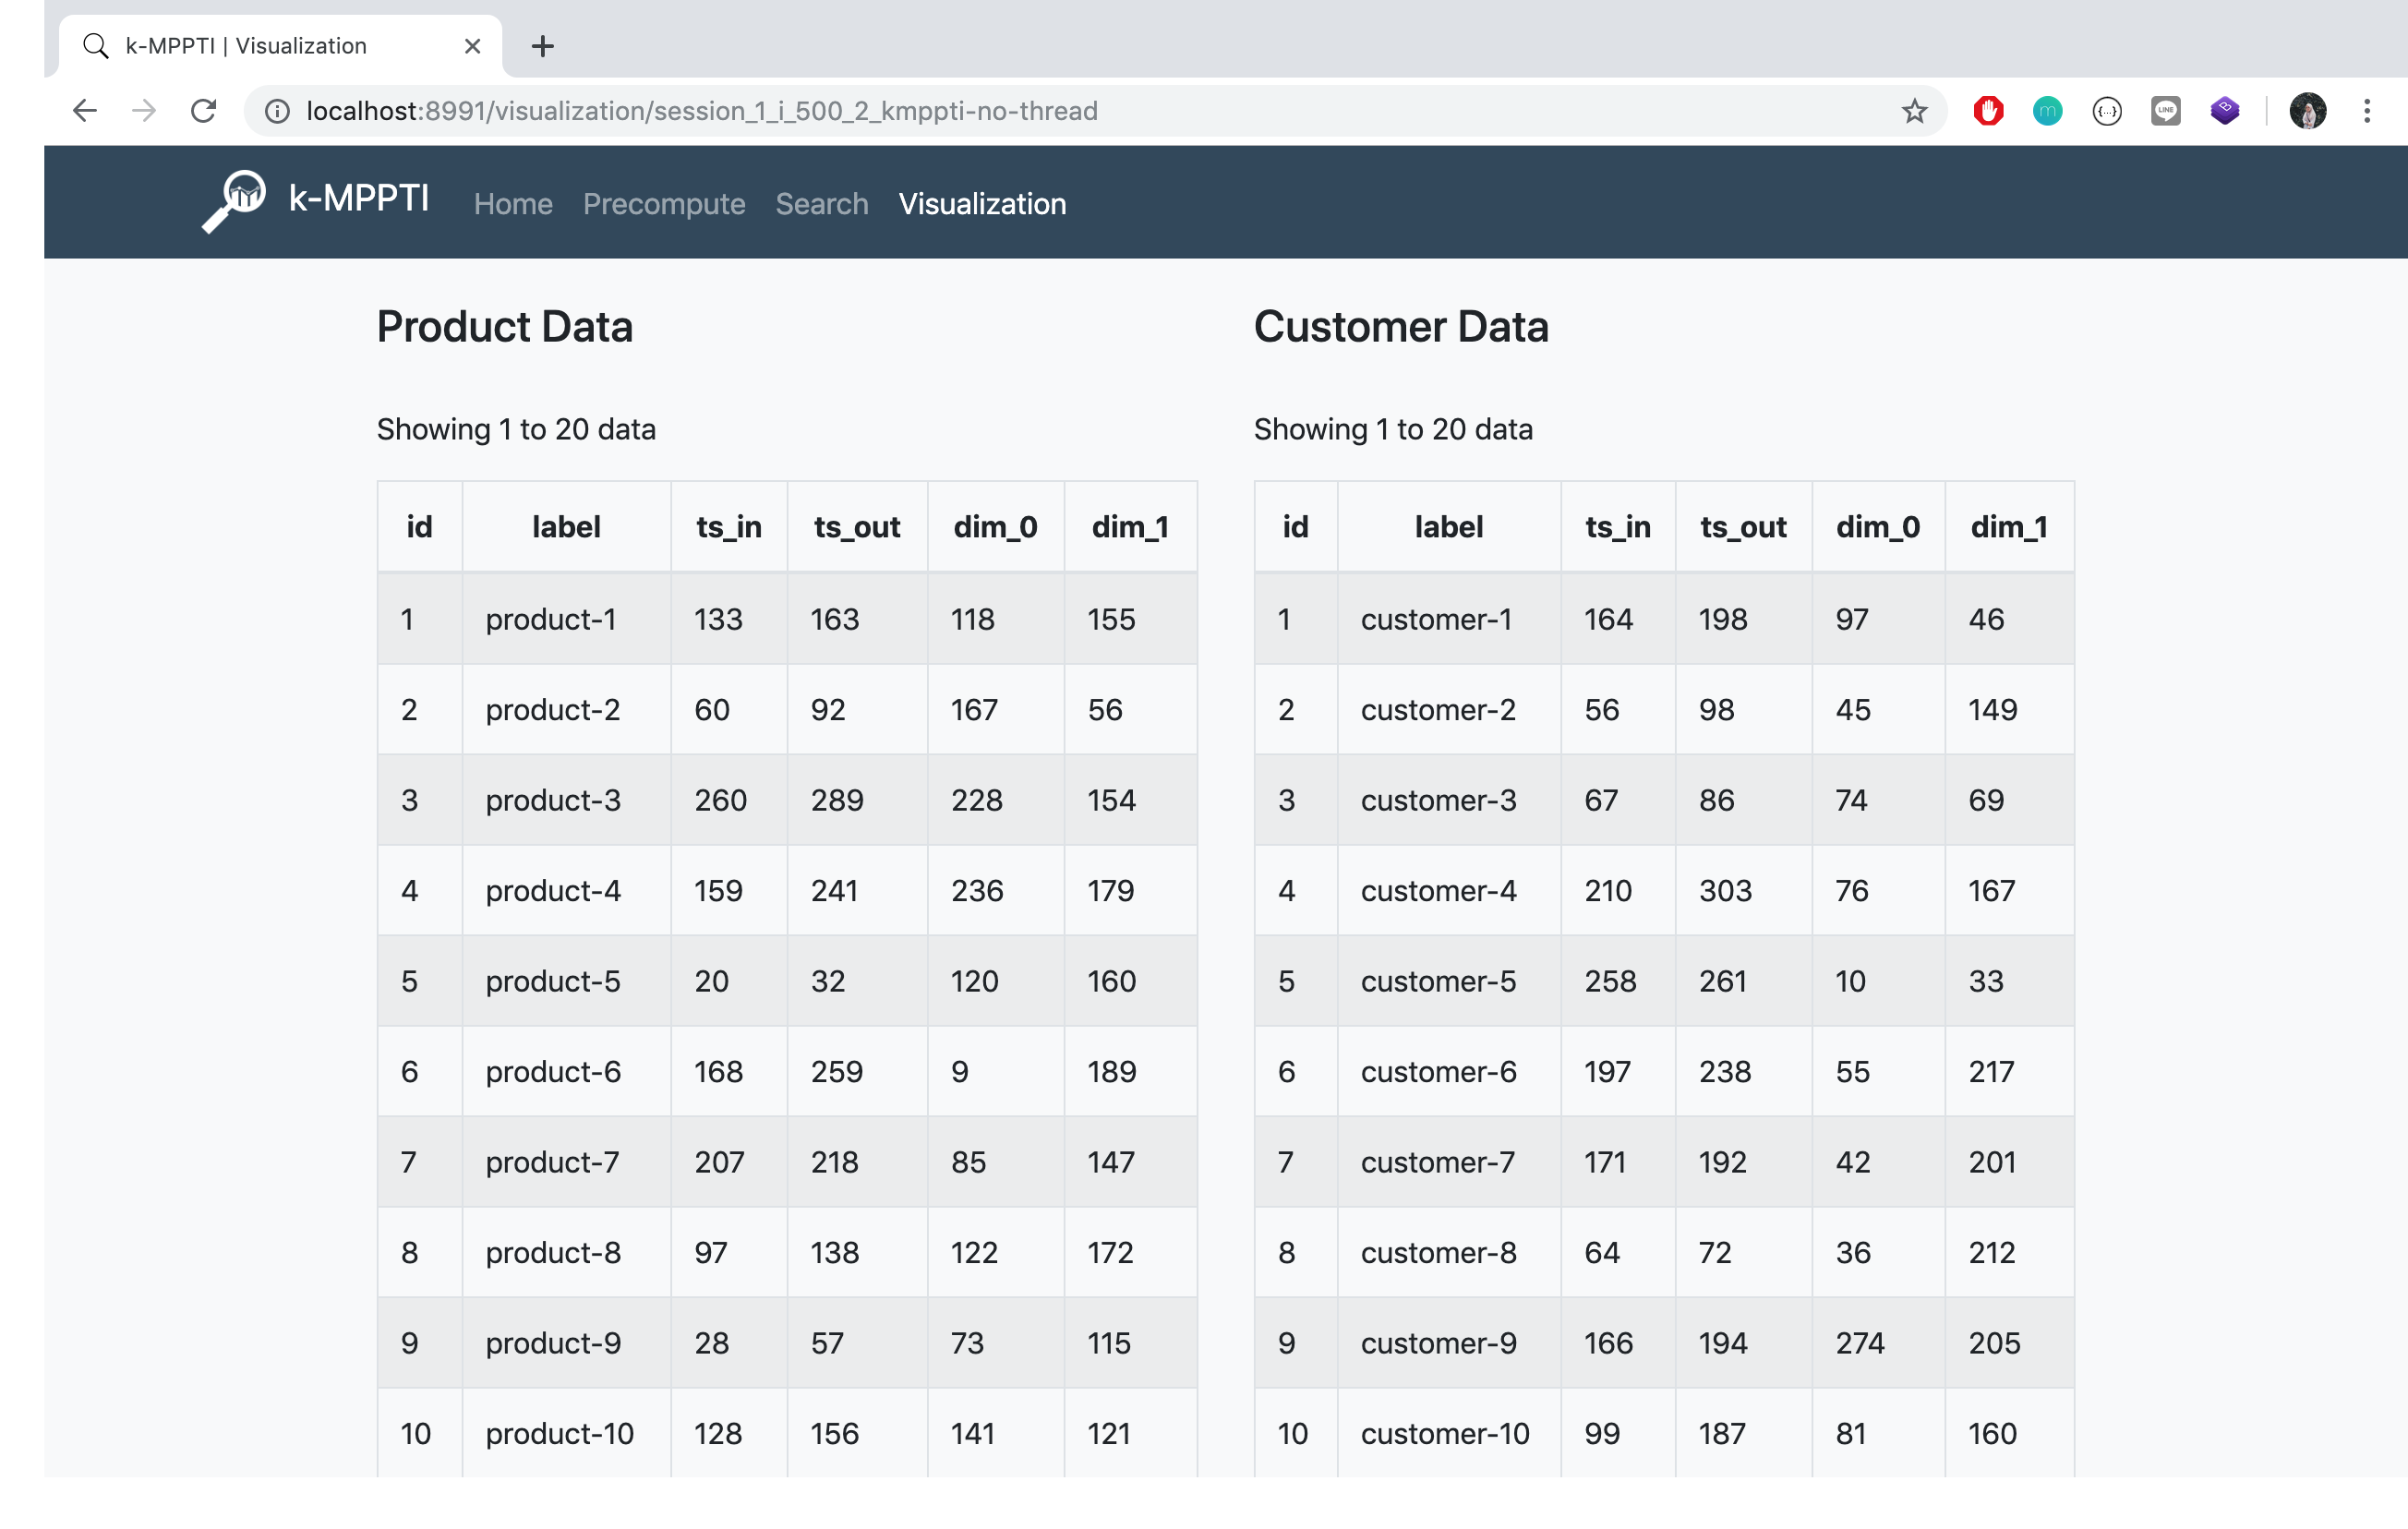
\includegraphics[width=8cm]{assets/img/bab4/visual-table.png}
	\caption{Implementasi Halaman \textit{Visualization} (Pratinjau Data Berbentuk Tabel)}
	\label{fig:visual-table}
\end{figure}

\begin{figure}[H]
	\centering
	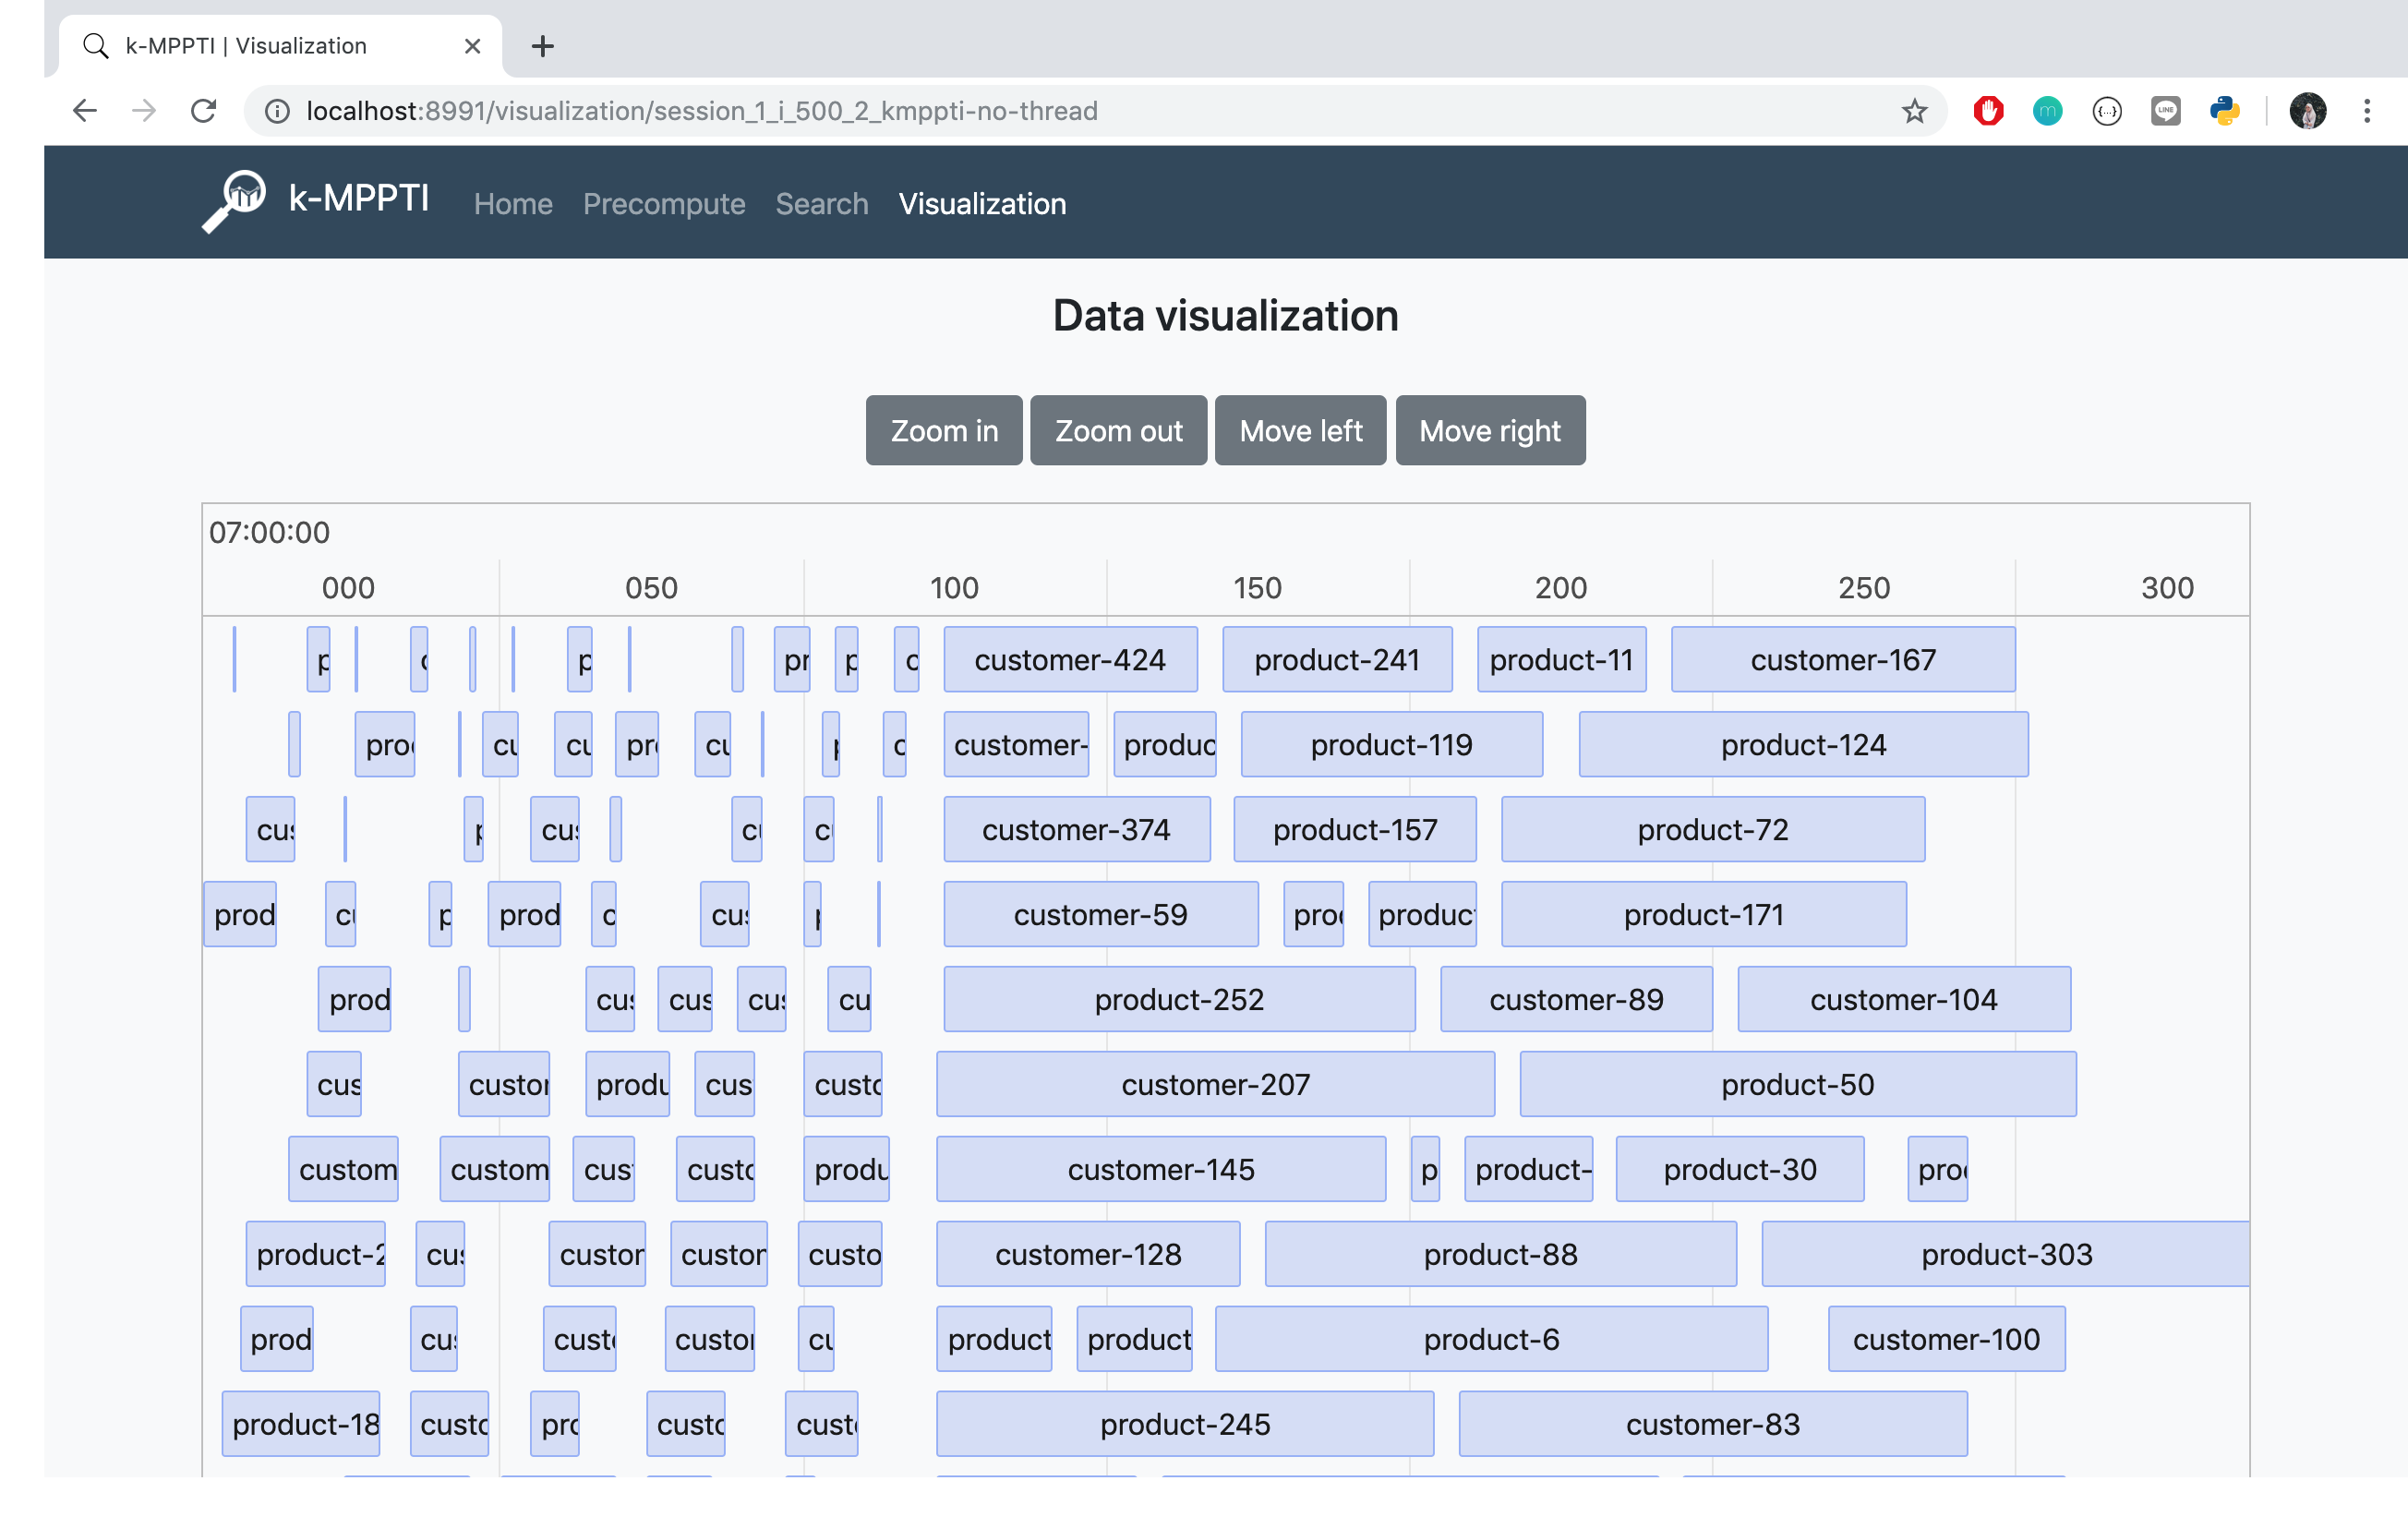
\includegraphics[width=8cm]{assets/img/bab4/visual-timeline.png}
	\caption{Implementasi Halaman \textit{Visualization} (Visualisasi Data Berbentuk Lini Masa)}
	\label{fig:visual-timeline}
\end{figure}